%==============================================================================%
% BAB 2: GAMBARAN UMUM PERUSAHAAN
%==============================================================================%

%-----------------------------------------------------------------------------%
\chapter{\babDua}

%-----------------------------------------------------------------------------%
\subsection{Deskripsi Perusahaan}

\begin{figure}[H]
\centering

\includegraphics[width=4cm]{assets/pics/logo_pns.png}
\caption{Logo PT Pratama Nusantara Sakti}
\label{fig:logo-perusahaan}
\end{figure}

Gambar \ref{fig:logo-perusahaan} menunjukkan logo resmi PT Pratama Nusantara Sakti, perusahaan tempat pelaksanaan kegiatan magang berlangsung.

\subsubsection{Sejarah Singkat Perusahaan}

\medskip

PT Pratama Nusantara Sakti merupakan perusahaan \textit{joint venture} yang
dibentuk atas kolaborasi strategis antara tiga kelompok usaha besar di Indonesia,
yaitu Djarum Group, Wings Group, dan CP Prima Group. Perusahaan ini bergerak di
bidang perkebunan tebu dan produksi gula, dengan wilayah operasional yang
berlokasi di Ogan Komering Ilir, Sumatera Selatan.

Perjalanan perusahaan dimulai pada tahun 2009 ketika PT Pratama Nusantara Sakti
resmi berdiri sebagai hasil sinergi ketiga kelompok usaha tersebut. Empat tahun
kemudian, pada tahun 2013, perusahaan memulai uji coba penanaman di lahan milik
perusahaan sebagai langkah strategis dalam mengembangkan praktik agrikultur yang
berkelanjutan. Momentum penting berikutnya terjadi pada tahun 2017, ketika
perusahaan melakukan peletakan batu pertama untuk pembangunan fasilitas pabrik,
dan konstruksi pabrik tersebut berhasil diselesaikan pada tahun 2019.

Memasuki tahun 2020, perusahaan berhasil melakukan \textit{commissioning} pabrik
untuk pertama kalinya, yang menandai pencapaian signifikan dalam perjalanan
operasional. Setahun kemudian, pada tahun 2021, PT Pratama Nusantara Sakti secara
resmi memulai produksi perdana, mencerminkan kesiapan penuh perusahaan untuk
memenuhi permintaan pasar. Komitmen terhadap kualitas agrikultur terus dibuktikan
pada tahun 2023, ketika perusahaan berhasil mencapai \textit{germination rate}
sebesar 88\%, sebuah indikator penting dalam keberhasilan program agrikultur
tebu yang dijalankan.

%-----------------------------------------------------------------------------%

\section{Struktur Organisasi Perusahaan}
%-----------------------------------------------------------------------------%

Dalam pelaksanaan kerja magang, posisi yang dijalankan adalah
\textit{Full-Stack Developer} di bawah pengawasan langsung supervisor atau
pembimbing lapangan yang bertugas memberikan arahan teknis dan mengevaluasi
progres mingguan. Koordinasi juga dilakukan secara aktif dengan klien dan tim
operasional lapangan, khususnya dalam hal validasi data tenaga kerja selama
proses migrasi dari sistem lama ke sistem baru.

\begin{figure}[h]
    \centering
    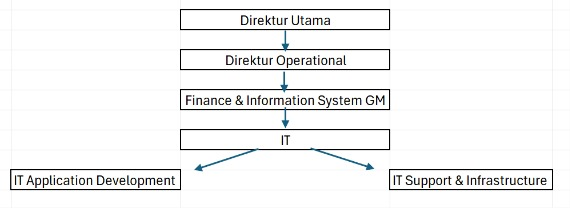
\includegraphics[width=0.9\textwidth]{assets/pics/fig_struktur-organisasi.jpg}
    \caption{Struktur Organisasi PT Pratama Nusantara Sakti}
    \label{fig:struktur-org}
\end{figure}


%-----------------------------------------------------------------------------%
% Landasan Teori dipindahkan ke berkas terpisah agar BAB 2 sesuai dengan
% template Career Acceleration Program v2026 (hanya Deskripsi Perusahaan &
% Struktur Organisasi). Untuk mengaktifkannya kembali, hapus komentar di bawah.
% %==============================================================================%
% LANDASAN TEORI (OPSIONAL)
%==============================================================================%
%
% CATATAN: Template 'Career Acceleration Program v2026' menyusun BAB 2 hanya
% dengan dua subbab: (2.1) Deskripsi Perusahaan dan (2.2) Struktur Organisasi
% Perusahaan -- TANPA subbab Landasan Teori.
%
% Agar laporan sesuai template, isi Landasan Teori dipindahkan ke berkas ini dan
% TIDAK dipanggil (tidak di-\input) dari Bab2.tex. Tidak ada tulisan yang hilang.
%
% Jika dosen pembimbing mengizinkan Landasan Teori tetap ada, cukup hapus tanda
% komentar pada baris \input berkas ini di bagian akhir src/2.Isi/Bab2.tex.
%==============================================================================%

%-----------------------------------------------------------------------------%
\section{Landasan Teori}
%-----------------------------------------------------------------------------%

Dalam mengembangkan aplikasi \textit{HR Safety Campus}, pemilihan tumpukan
teknologi (\textit{tech stack}) dan arsitektur keamanan sangat krusial untuk
menangani skala data belasan ribu pekerja secara efisien dan aman. Bagian ini
memaparkan dasar-dasar teori yang mendasari setiap keputusan teknis yang diambil
selama proses pengembangan berlangsung.

%-----------------------------------------------------------------------------%
\subsection{\textit{Human Resource Information System} (HRIS)}
%-----------------------------------------------------------------------------%

\textit{Human Resource Information System} (HRIS) adalah sistem terintegrasi
yang dirancang untuk mengelola, menyimpan, dan memproses data sumber daya manusia
dalam suatu organisasi secara terpusat dan terdigitalisasi \cite{almansouri2024hris}.
Secara konseptual, HRIS berfungsi sebagai jembatan antara kebutuhan administrasi
SDM dan kemampuan teknologi informasi, sehingga berbagai proses yang sebelumnya
dilakukan secara manual dapat diotomatiskan dengan lebih akurat dan efisien.

Almansouri et al. \cite{almansouri2024hris} menyebutkan bahwa implementasi HRIS
yang berhasil terbukti meningkatkan efisiensi operasional divisi HR secara
signifikan, antara lain melalui sentralisasi data karyawan, otomatisasi alur
persetujuan, serta pengurangan ketergantungan pada berkas fisik yang rentan
rusak atau hilang. Dalam konteks PT Pratama Nusantara Sakti, ketiga manfaat
tersebut menjadi inti dari pengembangan \textit{HR Safety Campus}: fitur
registrasi tenaga kerja mengotomatiskan pemberian ID karyawan, fitur klaim
transportasi mengotomatiskan perhitungan dan validasi nominal klaim, serta fitur
persetujuan karyawan mengotomatiskan \textit{workflow} yang sebelumnya dilakukan
secara manual oleh supervisor HR.

Lebih jauh, Susanti \cite{susanti2025hris} menunjukkan bahwa organisasi yang
sebelumnya mengandalkan alat seperti Microsoft Excel atau Microsoft Access untuk
pengelolaan SDM menghadapi tantangan yang serupa: data yang tersebar, validasi
yang lemah, dan sulitnya akses informasi secara \textit{real-time}. Temuan ini
memperkuat urgensi transformasi sistem di PT Pratama Nusantara Sakti dari
Microsoft Access ke platform berbasis web yang modern.

%-----------------------------------------------------------------------------%
\subsection{\textit{Role-Based Access Control} (RBAC)}
%-----------------------------------------------------------------------------%

Dalam sistem informasi sumber daya manusia yang mengelola data sensitif dan
klaim finansial, manajemen hak akses menjadi garis pertahanan utama terhadap
manipulasi data internal maupun oleh pihak vendor. \textit{Role-Based Access
Control} (RBAC) adalah mekanisme keamanan yang membatasi akses terhadap
sumber daya sistem berdasarkan peran (\textit{role}) spesifik yang dimiliki
oleh pengguna di dalam organisasi, bukan berdasarkan identitas individu semata
\cite{yuricha2023rbac}.

Prinsip inti dari RBAC adalah \textit{least privilege}, yaitu setiap pengguna
hanya diberikan izin akses seminimal mungkin yang dibutuhkan untuk menjalankan
tugasnya \cite{yuricha2023rbac}. Dalam konteks \textit{HR Safety Campus}, prinsip
ini diterapkan secara ketat: pengguna dengan peran Administrator memiliki otoritas
penuh untuk mengubah konfigurasi \textit{master data} tarif transportasi dan
mengelola akun pengguna lain, sementara pengguna dengan peran operasional di
lapangan hanya diberikan izin untuk melakukan registrasi karyawan atau mencetak
surat izin. Hal ini secara signifikan mereduksi risiko eskalasi hak istimewa
(\textit{privilege escalation}) dan menutup celah kecurangan pada proses klaim
transportasi \cite{mary2025rbac}.

Mary dan Febriyani \cite{mary2025rbac} secara khusus menunjukkan bahwa penerapan
RBAC pada kerangka kerja Laravel dapat diperkuat dengan lapisan keamanan tambahan
seperti \textit{rate limiting}, yang bersama-sama membentuk sistem pertahanan
berlapis terhadap akses tidak sah. Pendekatan ini sangat relevan mengingat
\textit{HR Safety Campus} menyimpan data pribadi ribuan tenaga kerja yang bersifat
sensitif dan berimplikasi langsung pada pengeluaran finansial perusahaan.

%-----------------------------------------------------------------------------%
\subsection{Pengembangan Antarmuka dengan \textit{Tailwind CSS}}
%-----------------------------------------------------------------------------%

Untuk mengimbangi kecepatan siklus pengembangan (\textit{development lifecycle})
di sisi peladen (\textit{backend}), diperlukan kerangka kerja antarmuka yang
menawarkan fleksibilitas tinggi tanpa mengorbankan konsistensi desain.
\textit{Tailwind CSS} adalah kerangka kerja CSS berbasis utilitas
(\textit{utility-first}) yang memungkinkan pengembang membangun antarmuka
langsung dari lapisan HTML tanpa perlu menulis berkas CSS khusus yang terpisah
\cite{nandan2024tailwind}.

Berbeda dengan kerangka kerja tradisional seperti Bootstrap yang menyediakan
komponen desain prasetel, Tailwind memberikan kendali yang sangat granular pada
level elemen HTML. Nandan et al. \cite{nandan2024tailwind} membuktikan melalui
pengujian empiris bahwa Tailwind CSS unggul dalam hal kustomisasi, fleksibilitas
desain, dan dukungan komunitas untuk proyek berskala besar yang memiliki komponen
UI yang beragam. Dalam konteks \textit{HR Safety Campus}, keunggulan ini
termanifestasi secara nyata: antarmuka sistem mencakup komponen yang sangat
bervariasi, mulai dari tabel data karyawan massal, formulir registrasi
multi-langkah, kartu surat izin, hingga lencana (\textit{badge}) status karyawan
yang kesemuanya dibangun dengan pendekatan \textit{utility-first} tanpa
membengkakkan basis kode CSS.

Lebih jauh lagi, implementasi Tailwind CSS pada sistem manajemen data berskala
besar terbukti mampu menjaga struktur kode tetap rapi serta mempertahankan
tingkat responsivitas yang tinggi di berbagai ukuran layar \cite{ardiyanto2023waterfall}.
Hal ini sangat krusial bagi tim IT di lapangan yang sering kali harus mengakses
modul registrasi atau persetujuan dokumen melalui perangkat yang bervariasi,
mulai dari komputer meja di kantor hingga \textit{laptop} di lokasi lapangan.

%-----------------------------------------------------------------------------%
\subsection{Deteksi dan Penanganan Duplikasi Data (\textit{Data Deduplication})}
%-----------------------------------------------------------------------------%

Salah satu tantangan teknis terbesar yang dihadapi dalam proyek ini adalah
deteksi dan penanganan data yang terduplikasi dalam basis data berskala besar.
\textit{Data deduplication} adalah proses identifikasi dan eliminasi rekaman
data yang berulang dalam suatu basis data, dengan tujuan menjaga integritas dan
akurasi informasi yang tersimpan \cite{ravikanth2024deduplication}.

Ravikanth et al. \cite{ravikanth2024deduplication} menjelaskan bahwa duplikasi
data dalam sistem informasi karyawan dapat terjadi karena berbagai sebab: kesalahan
entri manual yang berlangsung bertahun-tahun, seorang karyawan yang keluar lalu
kembali bergabung dan didaftarkan ulang tanpa merujuk data lama, atau data yang
disalin tanpa melalui proses validasi. Pada proses migrasi data di PT Pratama
Nusantara Sakti, kondisi ini terjadi secara nyata: dari sekitar 4.000 rekaman
yang diidentifikasi, ditemukan duplikasi pada kolom NIK yang seharusnya bersifat
unik, sehingga proses unggah data (\textit{upload}) ke MySQL gagal karena
melanggar aturan integritas basis data (\textit{database integrity constraint}).

Untuk menangani permasalahan ini, dibangun skrip seleksi data khusus yang
memisahkan rekaman ganda sebelum dilakukan pembersihan menggunakan perintah
\texttt{TRUNCATE} dan pengunggahan ulang berkas CSV yang telah dibersihkan.
Selain itu, mekanisme \textit{Re-Hire} yang terintegrasi dalam fitur registrasi
turut dirancang untuk mencegah duplikasi di masa mendatang: ketika petugas
mencoba mendaftarkan NIK yang pernah terdaftar sebelumnya, sistem akan
mendeteksinya secara otomatis dan menawarkan opsi pemulihan data lama daripada
membuat rekaman baru yang redundan.

%-----------------------------------------------------------------------------%
\subsection{Metode Pengembangan Perangkat Lunak \textit{Waterfall}}
%-----------------------------------------------------------------------------%

Pengembangan sistem \textit{HR Safety Campus} dilaksanakan menggunakan pendekatan
metode \textit{Waterfall}, yaitu model pengembangan perangkat lunak yang bersifat
sekuensial dan terstruktur. Dalam metode ini, setiap fase pengembangan diselesaikan
secara tuntas sebelum melanjutkan ke fase berikutnya, sehingga setiap tahapan
memiliki keluaran (\textit{deliverable}) yang jelas dan terverifikasi
\cite{ardiyanto2023waterfall}.

Ardiyanto et al. \cite{ardiyanto2023waterfall} menunjukkan bahwa metode
\textit{Waterfall} sangat sesuai diterapkan pada proyek pengembangan sistem
informasi karyawan berbasis web yang memiliki ruang lingkup dan kebutuhan yang
sudah terdefinisi dengan baik sejak awal. Tahapan dalam metode ini meliputi
analisis kebutuhan, perancangan sistem, implementasi kode, pengujian
fungsionalitas, serta pemeliharaan. Kesesuaian ini tercermin dalam
pelaksanaan magang di PT Pratama Nusantara Sakti, di mana pengembangan dimulai
dari observasi mendalam terhadap sistem lama, dilanjutkan dengan perancangan
solusi, implementasi bertahap selama 20 minggu, hingga evaluasi akhir dan
penyerahan dokumentasi.
%-----------------------------------------------------------------------------%
\subsection{Arsitektur \textit{Model-View-Controller} (MVC) pada Laravel}
%-----------------------------------------------------------------------------%

Kerangka kerja Laravel yang digunakan dalam pengembangan \textit{HR Safety
Campus} mengadopsi pola arsitektur \textit{Model-View-Controller} (MVC), yaitu
pola perancangan yang memisahkan logika aplikasi menjadi tiga komponen utama:
\textit{Model} yang menangani logika data dan interaksi dengan basis data,
\textit{View} yang bertanggung jawab atas penyajian antarmuka, serta
\textit{Controller} yang menjembatani keduanya dengan mengatur alur permintaan
dan respons \cite{rahmawati2024mvc}. Rahmawati dan Sumarsono
\cite{rahmawati2024mvc} menunjukkan bahwa penerapan pola MVC pada Laravel
membantu menjaga kode tetap terstruktur dan mempermudah pemeliharaan
berkelanjutan, sebuah keunggulan yang sangat relevan untuk proyek dengan banyak
modul seperti \textit{HR Safety Campus}.

Selain kerapian struktur kode, pemilihan Laravel juga didasari pertimbangan
performa dan produktivitas dalam pengembangan lapisan komunikasi data. Ariyanto
et al. \cite{ariyanto2024restapi} melalui pengujian komparatif membuktikan
bahwa pengembangan \textit{REST API} menggunakan Laravel menghasilkan struktur
kode yang lebih ringkas, terpelihara, dan mudah dikembangkan dibandingkan
pendekatan PHP \textit{native}. Dalam konteks \textit{HR Safety Campus}, fasilitas
bawaan Laravel seperti \textit{routing}, \textit{Eloquent ORM}, dan sistem migrasi
basis data dimanfaatkan secara intensif untuk menangani integrasi data wilayah
IndoRegion serta sinkronisasi data tenaga kerja berskala ribuan rekaman.

%-----------------------------------------------------------------------------%
